\documentclass{article}
\usepackage{tikz}
\usetikzlibrary{graphs, quotes, arrows.meta}
\begin{document}

\begin{figure}[h]
\centering
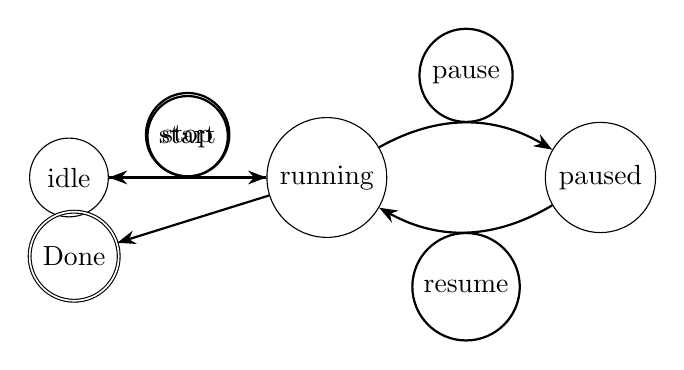
\begin{tikzpicture}[>=Stealth, every node/.style={circle, draw, minimum size=1cm}]
  \graph[grow right sep=2cm, edges={thick}] {
    idle ->["start"] running ->["pause", bend left] paused ->["resume", bend left] running;
    running ->["stop"'] idle;
    running -> done/"Done"[double];
  };
\end{tikzpicture}
\caption{Process states.}
\end{figure}

\begin{figure}[h]
\centering
\tikz \graph [circular placement, radius=1.5cm, nodes={draw, circle, fill=gray!20}] {
  subgraph K_n [n=5]
};
\quad
\tikz \graph [clockwise, radius=1.2cm, empty nodes, nodes={fill, circle, inner sep=2pt}] {
  subgraph C_n [n=6]
};
\caption{The complete graph $K_5$ and the cycle $C_6$.}
\end{figure}

\end{document}
